\chapter{Гиперболические функции}\label{chap:c14-hyperbolic}\markright{Глава 27}
\section{Гиперболические функции}
\begin{definition}\term{Гиперболический синус} (hyperbolic sine) — функция \(\operatorname{sh} x=\frac{e^x-e^{-x}}2\), определённая для всех действительных \(x\).\end{definition}
\begin{definition}\term{Гиперболический косинус} (hyperbolic cosine) — функция \(\operatorname{ch} x=\frac{e^x+e^{-x}}2\), определённая для всех действительных \(x\).\end{definition}
\begin{theorem}[Основное тождество и чётность]\label{thm:legacy-c14-3}
Для любого действительного \(x\) выполнено \(\operatorname{ch}^2x-\operatorname{sh}^2x=1\), \(\operatorname{sh}(-x)=-\operatorname{sh} x\), \(\operatorname{ch}(-x)=\operatorname{ch} x\).
\end{theorem}
\begin{proof}
Вычитаем квадраты по определениям: \(\operatorname{ch}^2x-\operatorname{sh}^2x=\frac{(e^x+e^{-x})^2-(e^x-e^{-x})^2}{4}=e^xe^{-x}=1\). При замене \(x\) на \(-x\) два слагаемых в числителях меняются местами: разность меняет знак, а сумма сохраняется. Это доказывает обе формулы чётности.
\end{proof}
\section{Гиперболические тангенс и котангенс}
\begin{definition}\term{Гиперболический тангенс} (\emph{hyperbolic tangent}) — функция \(\operatorname{th}x=\frac{\operatorname{sh}x}{\operatorname{ch}x}\), \(x\in\mathbb R\). Знаменатель всегда положителен. В англоязычной литературе обычно пишут \(\tanh x\).\end{definition}
\begin{definition}\term{Гиперболический котангенс} (\emph{hyperbolic cotangent}) — функция \(\operatorname{cth}x=\frac{\operatorname{ch}x}{\operatorname{sh}x}\), \(x\ne0\). В англоязычной литературе обычно пишут \(\coth x\).\end{definition}
\begin{theorem}[Рациональные выражения через экспоненту]\label{thm:legacy-c14-4}
При \(t=e^{2x}>0\) имеем
\[
\operatorname{th}x=\frac{t-1}{t+1},\qquad
\operatorname{cth}x=\frac{t+1}{t-1}\quad(x\ne0).
\]
Обе функции нечётны. Множество значений \(\operatorname{th}\) равно \((-1;1)\), а \(\operatorname{cth}\) — \((-\infty;-1)\cup(1;+\infty)\).
\end{theorem}
\begin{proof}
Подставим определения \(\operatorname{sh}\), \(\operatorname{ch}\) и умножим числитель и знаменатель на \(e^x\). Нечётность следует из нечётности \(\operatorname{sh}\) и чётности \(\operatorname{ch}\). При \(t>0\) выполнено \(|t-1|<t+1\), что даёт указанные строгие границы. Обратно, для \(-1<y<1\) число \(t=\frac{1+y}{1-y}>0\) даёт \(\operatorname{th}(\frac12\ln t)=y\). При \(|y|>1\) число \(t=\frac{y+1}{y-1}>0\) отлично от \(1\) и даёт \(\operatorname{cth}(\frac12\ln t)=y\). Поэтому все указанные значения достигаются.
\end{proof}
\par\addvspace{5pt}\begin{lrbox}{\CatFlowBox}\begin{minipage}[t]{\linewidth}
\setlength{\parskip}{5pt}\setlength{\columnsep}{4.5mm}\setlength{\intextsep}{0pt}
\begin{wrapfigure}[11]{l}{54mm}

\includegraphics[width=54mm,height=58mm,keepaspectratio]{images/unique/art-97.png}
\end{wrapfigure}
Гиперболический тангенс ограничен, хотя его аргумент может расти без границ. Например, заданная модель сигнала \(s(t)=2\operatorname{th}t\) всегда даёт \(-2<s(t)<2\). Значения приближаются к границам, но не достигают их при конечном \(t\). В отличие от обычного тангенса, у \(\operatorname{th}\) на действительной прямой нет полюсов и нет ненулевого периода. У \(\operatorname{cth}\) область определения разрывается в нуле; это нужно учитывать до сокращения выражений и решения уравнений. Периодические ветви обычного котангенса и две ветви гиперболического котангенса имеют разное происхождение.
\par\WFclear\end{minipage}\end{lrbox}%
\ifdim\dimexpr\ht\CatFlowBox+\dp\CatFlowBox\relax<64mm\dp\CatFlowBox=\dimexpr64mm-\ht\CatFlowBox\relax\fi%
\noindent\usebox{\CatFlowBox}\par\addvspace{5pt}
\begin{theorem}[Тождества и монотонность]\label{thm:legacy-c14-5}
Для действительного \(x\) выполнено \(1-\operatorname{th}^2x=\frac1{\operatorname{ch}^2x}\); при \(x\ne0\) — \(\operatorname{cth}^2x-1=\frac1{\operatorname{sh}^2x}\). Функция \(\operatorname{th}\) строго возрастает на \(\mathbb R\), а \(\operatorname{cth}\) строго убывает на каждом из промежутков \((-\infty;0)\), \((0;+\infty)\).
\end{theorem}
\begin{proof}
Разделим равенство \(\operatorname{ch}^2x-\operatorname{sh}^2x=1\) соответственно на \(\operatorname{ch}^2x\) и \(\operatorname{sh}^2x\). Для монотонности пусть \(0<t_1<t_2\). Разность значений \(\frac{t-1}{t+1}\) равна \(\frac{2(t_2-t_1)}{(t_2+1)(t_1+1)}>0\). Разность значений \(\frac{t+1}{t-1}\) равна \(-\frac{2(t_2-t_1)}{(t_2-1)(t_1-1)}<0\), если \(t_1,t_2\) лежат по одну сторону от \(1\). Экспонента \(e^{2x}\) строго возрастает, что даёт все утверждения. Неограниченность аргумента и строгая монотонность также исключают ненулевой период \(\operatorname{th}\).
\end{proof}

\section{Зачем нужны гиперболические функции}
В геометрии параметризация \(X=\operatorname{ch}t\), \(Y=\operatorname{sh}t\) даёт точки правой ветви гиперболы \(X^2-Y^2=1\), поскольку \(\operatorname{ch}t>0\). Это аналог связи косинуса и синуса с окружностью, но с разностью квадратов вместо суммы.

\par\addvspace{5pt}\begin{lrbox}{\CatFlowBox}\begin{minipage}[t]{\linewidth}
\setlength{\parskip}{5pt}\setlength{\columnsep}{4.5mm}\setlength{\intextsep}{0pt}
\begin{wrapfigure}[11]{r}{54mm}

\includegraphics[width=54mm,height=58mm,keepaspectratio]{images/unique/art-93.png}
\end{wrapfigure}
Другая модель — цепная линия (\emph{catenary}). Идеальная гибкая однородная нерастяжимая цепь в равновесии под собственным весом в однородном поле тяжести, подвешенная за концы на одинаковой высоте, при подходящем выборе координат имеет профиль
\[
y=a\left(\operatorname{ch}\frac xa-1\right),\qquad a>0.
\]
Оси \(x,y\) и параметр \(a\) измеряются в единицах длины, поэтому аргумент \(\frac xa\) безразмерен. Начало координат расположено в нижней точке цепи. Например, при \(a=2\) м и \(x=2\ln2\) м получаем \(y=2(\frac{2+\frac12}{2}-1)=\frac12\) м. Вывод физической модели требует механики; здесь мы исследуем заданную функцию.

У модели минимум \(y=0\) при \(x=0\): для \(u=e^t>0\) неравенство \(u+\frac1u\ge2\) следует из \(\frac{(u-1)^2}{u}\ge0\). Значит, \(\operatorname{ch}t\ge1\), причём равенство возможно только при \(t=0\). График симметричен относительно вертикальной оси по чётности \(\operatorname{ch}\).
\par\WFclear\end{minipage}\end{lrbox}%
\ifdim\dimexpr\ht\CatFlowBox+\dp\CatFlowBox\relax<64mm\dp\CatFlowBox=\dimexpr64mm-\ht\CatFlowBox\relax\fi%
\noindent\usebox{\CatFlowBox}\par\addvspace{5pt}
% HYPERBOLIC_APPLICATION_END
График \(\operatorname{sh} x\) нечётен, строго возрастает и проходит через \((0;0)\). Возрастание видно без производных: при \(y>x\) одновременно \(e^y>e^x\) и \(-e^{-y}>-e^{-x}\). График \(\operatorname{ch} x\) чётен и проходит через \((0;1)\); его наименьшее значение равно \(1\). Для \(0\le x<y\) равенство \(\operatorname{ch} y-\operatorname{ch} x=2\operatorname{sh}\frac{y+x}{2}\operatorname{sh}\frac{y-x}{2}>0\), получаемое раскрытием определений, показывает возрастание на \([0;+\infty)\); из чётности следует убывание на \((-\infty;0]\). Таким образом, график имеет плавную форму цепи с минимумом в \((0;1)\), но не совпадает с параболой.


\par\noindent\begin{minipage}{\linewidth}\section*{Графики}
\begin{center}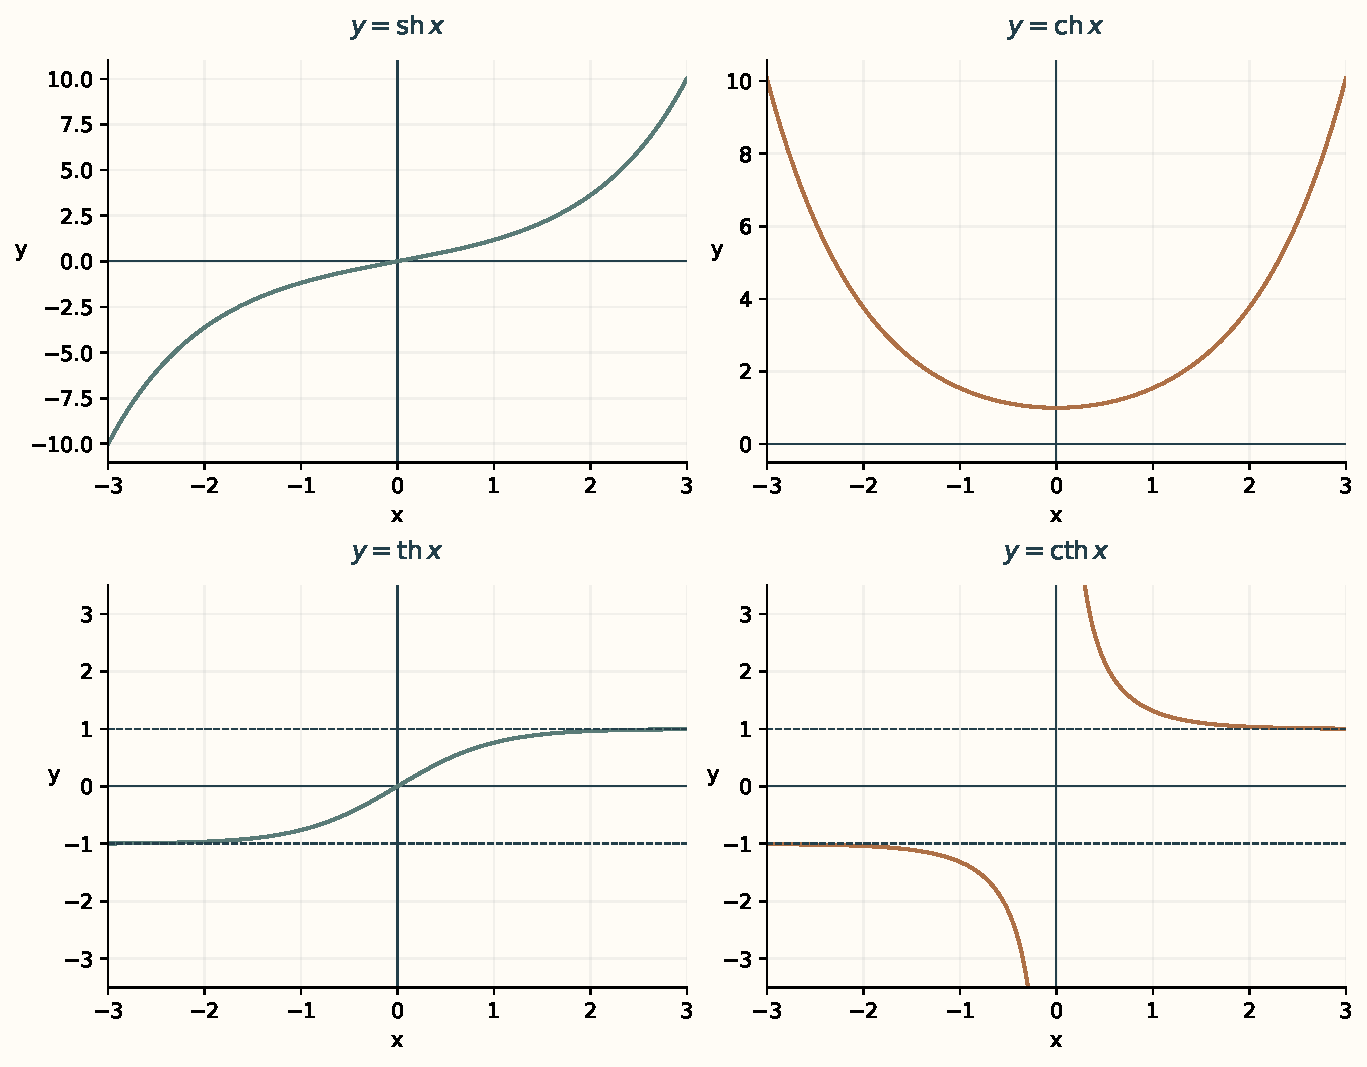
\includegraphics[width=\textwidth,height=.79\textheight,keepaspectratio]{images/atlas-hyperbolic-all.pdf}\par\small Гиперболические функции\end{center}\end{minipage}\par
\Needspace{7\baselineskip}\section*{Задачи}
\begingroup\setlength{\parskip}{2pt}
\noindent\begin{minipage}[t]{\linewidth}\textbf{27.1.}\starmark{} Докажи, что \(\operatorname{ch} x\ge1\) для всех действительных \(x\). При каком \(x\) достигается равенство? Используй квадрат разности \(e^{x/2}-e^{-x/2}\).\par\end{minipage}\par
\noindent\begin{minipage}[t]{\linewidth}\textbf{27.2.} Вычисли в точном виде \(\operatorname{sh}(\ln2)\) и \(\operatorname{ch}(\ln2)\). Проверь для этих значений основное гиперболическое тождество.\par\end{minipage}\par
\noindent\begin{minipage}[t]{\linewidth}\textbf{27.3.}\starmark{} Реши \(\operatorname{sh} x=\dfrac34\), сделав замену \(t=e^x\). Укажи допустимые значения \(t\).\par\end{minipage}\par
\noindent\begin{minipage}[t]{\linewidth}\textbf{27.4.}\starmark{} Реши \(\operatorname{ch} x=\dfrac54\), используя определения гиперболических функций.\par\end{minipage}\par
\noindent\begin{minipage}[t]{\linewidth}\textbf{27.5.} Построй эскизы графиков \(y=\operatorname{sh} x\) и \(y=\operatorname{ch} x\) в одной системе координат. Используй точки с аргументами \(-\ln2\), \(0\), \(\ln2\); отметь чётность и положение графиков относительно оси абсцисс.\par\end{minipage}\par
\noindent\begin{minipage}[t]{\linewidth}\textbf{27.6.} В модели цепи \(y=4(\operatorname{ch}\dfrac x4-1)\) все длины даны в метрах. Найди высоту при \(x=4\ln2\), а также высоту в симметричной точке.\par\end{minipage}\par
\noindent\begin{minipage}[t]{\linewidth}\textbf{27.7.}\starmark{} Докажи, что профиль \(y=a(\operatorname{ch}\dfrac xa-1)\), \(a>0\), достигает единственного минимума в нуле. Используй определения, без производной.\par\end{minipage}\par
\noindent\begin{minipage}[t]{\linewidth}\textbf{27.8.} На гиперболе задана точка \((X,Y)=(\operatorname{ch}t,\operatorname{sh}t)\), где \(t=\ln3\). Найди координаты и проверь \(X^2-Y^2=1\).\par\end{minipage}\par
\par\addvspace{5pt}\begin{lrbox}{\CatFlowBox}\begin{minipage}[t]{\linewidth}
\setlength{\parskip}{5pt}\setlength{\columnsep}{4.5mm}\setlength{\intextsep}{0pt}
\begin{wrapfigure}[13]{r}{54mm}

\includegraphics[width=54mm,height=58mm,keepaspectratio]{images/unique/art-132.png}
\end{wrapfigure}
\textbf{27.9.} Найди \(\operatorname{th}0\), \(\operatorname{th}(\ln2)\), \(\operatorname{cth}(\ln2)\).\par

\textbf{27.10.} Вычисли \(\operatorname{th}(-\ln3)\) и \(\operatorname{cth}(-\ln3)\).\par

\textbf{27.11.} Реши \(\operatorname{th}x=\dfrac12\) на действительной прямой.\par

\textbf{27.12.} Реши \(\operatorname{cth}x=2\), проверив область определения.\par
\par\WFclear\end{minipage}\end{lrbox}%
\ifdim\dimexpr\ht\CatFlowBox+\dp\CatFlowBox\relax<64mm\dp\CatFlowBox=\dimexpr64mm-\ht\CatFlowBox\relax\fi%
\noindent\usebox{\CatFlowBox}\par\addvspace{5pt}

\noindent\begin{minipage}[t]{\linewidth}\textbf{27.13.} Какие из уравнений \(\operatorname{th}x=1\), \(\operatorname{th}x=-\dfrac32\), \(\operatorname{cth}x=\dfrac12\) имеют действительные решения?\par\end{minipage}\par
\noindent\begin{minipage}[t]{\linewidth}\textbf{27.14.} Построй эскизы \(y=\operatorname{th}x\) и \(y=\operatorname{cth}x\). Отметь область определения, нечётность и горизонтальные асимптоты.\par\end{minipage}\par
\noindent\begin{minipage}[t]{\linewidth}\textbf{27.15.} В заданной модели \(s(t)=2\operatorname{th}t\) найди момент \(t\ge0\), когда \(s(t)=1\), и объясни, достигается ли уровень \(2\).\par\end{minipage}\par
\noindent\begin{minipage}[t]{\linewidth}\textbf{27.16.} Докажи \(\operatorname{cth}x\operatorname{th}x=1\). Укажи все допустимые \(x\).\par\end{minipage}\par
\noindent\begin{minipage}[t]{\linewidth}\textbf{27.17.}\starmark{} Докажи формулу \(\operatorname{th}(x+y)=\dfrac{\operatorname{th}x+\operatorname{th}y}{1+\operatorname{th}x\operatorname{th}y}\). Почему знаменатель ненулевой?\par\end{minipage}\par
\noindent\begin{minipage}[t]{\linewidth}\textbf{27.18.}\starmark{} При \(a>0\) реши неравенство \(|\operatorname{th}x|\le\operatorname{th}a\).\par\end{minipage}\par
\endgroup
